\documentclass[11pt,a4paper]{article}

% xcolor (loaded by macros_FP) and the later color package clash unless the
% options are declared up front; this keeps macros_FP.tex untouched.
\PassOptionsToPackage{usenames,dvipsnames}{color}
% start of paragraph with no indent
\parindent0pt

% insert packages in alphabetical order
\usepackage{algorithm, algpseudocode, amssymb, amsthm, bbm, csquotes, docmute, enumitem, float, geometry, graphicx, hyphenat, listings, mathtools, physics, tcolorbox, tikz, tocloft, xcolor, natbib}
\usepackage[english]{babel}

% load packages
\usepackage{geometry}
 \geometry{
 a4paper,
 total={170mm,257mm},
 left=20mm,
 top=20mm,
 }
\usepackage{amsfonts}
\usepackage[usenames, dvipsnames]{color}
%\usepackage{bbold}
%\usepackage{url}
\usepackage{upgreek}
\usepackage{placeins}
\usepackage{empheq}
\usepackage{tabularx}
\usepackage{booktabs}
\definecolor{red}{RGB}{255, 0, 0}
\usepackage{tabto}
\usepackage{tgtermes,tgheros} 
\usepackage{enumitem}% http://ctan.org/pkg/enumitem
\usepackage{titlesec}
\usepackage{hyperref}

\titleformat{\section}[block]
  {\fontsize{12}{15}\bfseries\sffamily\filcenter}
  {\thesection}
  {1em}
  {\MakeUppercase}
\titleformat{\subsection}[hang]
  {\fontsize{12}{15}\bfseries\sffamily}
  {\thesubsection}
  {1em}
  {}

\allowdisplaybreaks

% math symbols
\newcommand{\bA}{\mathbb{A}}
\newcommand{\bB}{\mathbb{B}}
\newcommand{\bC}{\mathbb{C}}
\newcommand{\bD}{\mathbb{D}}
\newcommand{\bE}{\mathbb{E}}
\newcommand{\bF}{\mathbb{F}}
\newcommand{\bG}{\mathbb{G}}
\newcommand{\bH}{\mathbb{H}}
\newcommand{\bI}{\mathbb{I}}
\newcommand{\bJ}{\mathbb{J}}
\newcommand{\bK}{\mathbb{K}}
\newcommand{\bL}{\mathbb{L}}
\newcommand{\bM}{\mathbb{M}}
\newcommand{\bN}{\mathbb{N}}
\newcommand{\bO}{\mathbb{O}}
\newcommand{\bP}{\mathbb{P}}
\newcommand{\bQ}{\mathbb{Q}}
\newcommand{\bR}{\mathbb{R}}
\newcommand{\bS}{\mathbb{S}}
\newcommand{\bT}{\mathbb{T}}
\newcommand{\bU}{\mathbb{U}}
\newcommand{\bV}{\mathbb{V}}
\newcommand{\bW}{\mathbb{W}}
\newcommand{\bX}{\mathbb{X}}
\newcommand{\bY}{\mathbb{Y}}
\newcommand{\bZ}{\mathbb{Z}}

\NewDocumentCommand{\codeword}{v}{%
\texttt{\textcolor{blue}{#1}}%
}


\newcommand{\cA}{\mathcal{A}}
\newcommand{\cB}{\mathcal{B}}
\newcommand{\cC}{\mathcal{C}}
\newcommand{\cD}{\mathcal{D}}
\newcommand{\cE}{\mathcal{E}}
\newcommand{\cF}{\mathcal{F}}
\newcommand{\cG}{\mathcal{G}}
\newcommand{\cH}{\mathcal{H}}
\newcommand{\cI}{\mathcal{I}}
\newcommand{\cJ}{\mathcal{J}}
\newcommand{\cK}{\mathcal{K}}
\newcommand{\cL}{\mathcal{L}}
\newcommand{\cM}{\mathcal{M}}
\newcommand{\cN}{\mathcal{N}}
\newcommand{\cO}{\mathcal{O}}
\newcommand{\cP}{\mathcal{P}}
\newcommand{\cQ}{\mathcal{Q}}
\newcommand{\cR}{\mathcal{R}}
\newcommand{\cS}{\mathcal{S}}
\newcommand{\cT}{\mathcal{T}}
\newcommand{\cU}{\mathcal{U}}
\newcommand{\cV}{\mathcal{V}}
\newcommand{\cW}{\mathcal{W}}
\newcommand{\cX}{\mathcal{X}}
\newcommand{\cY}{\mathcal{Y}}
\newcommand{\cZ}{\mathcal{Z}}
\newcommand{\vect}[1]{\mathbf{#1}}

\newcommand{\e}{\text{e}}

\newcommand{\ber}{\text{Ber}}
\newcommand{\bin}{\text{Bin}}
\newcommand{\poi}{\text{Poi}}
\newcommand{\geo}{\text{Geo}}
\newcommand{\Exp}{\text{Exp}}

\newcommand{\cov}{\text{Cov}}
\newcommand{\corr}{\rho}
\newcommand{\risk}{\text{R}}
\newcommand{\bias}{\text{Bias}}
\newcommand{\mse}{\text{MSE}}
\newcommand{\se}{\text{SE}}
\newcommand{\elbo}{\text{ELBO}}
\newcommand{\kl}{\text{KL}}

\newcommand{\acov}{\text{acov}}
\newcommand{\acorr}{\text{acorr}}
\newcommand{\xcov}{\text{xcov}}
\newcommand{\xcorr}{\text{xcorr}}
\newcommand{\pacorr}{\text{pacorr}}
\newcommand{\pacov}{\text{pacov}}

\newcommand{\relu}{\text{ReLU}}

\newcommand{\deriv}[2]{\frac{\partial #1}{\partial #2}}

\DeclareMathOperator*{\argmax}{arg\,max}
\DeclareMathOperator*{\argmin}{arg\,min}

% math environments
\theoremstyle{definition}
\newtheorem{definition}{Definition}[section]
\newtheorem{theorem}[definition]{Theorem}
\newtheorem{proposition}[definition]{Proposition}
\newtheorem{example}[definition]{Example}
\newtheorem{remark}[definition]{Remark}
\newtheorem{task}[definition]{Task}

\newenvironment{boxedtheorem}[1][]
{\begin{tcolorbox}[colback=white!95!gray, colframe=black, title=#1]}
{\end{tcolorbox}}

\newenvironment{boxeddefinition}[1][]
{\begin{tcolorbox}[colback=white, colframe=grey, title=#1]}
{\end{tcolorbox}}



% macros_FP sets \parindent0pt and no \parskip, which leaves paragraph breaks invisible.
% A first-line indent restores them at zero cost in vertical space. hidelinks removes the
% coloured boxes hyperref otherwise draws around every citation. Neither alters the page
% geometry, the font size or the line spacing.
\setlength{\parindent}{1.2em}
\hypersetup{hidelinks}

\begin{document}

\begin{center}
{\Large\bfseries Conflict, not confidence: which value\,$\to$\,RT mapping\\[2pt]
best describes probability discounting, and does RT help?}\\[6pt]
Computational Cognitive Science --- Final Project, Summer Term 2026\\[8pt]

\begin{tabular}{lll}
\textbf{Name} & \textbf{Matriculation no.} & \textbf{Contribution}\\
\hline
Ashhad Raza Quadri & 4756039 & M1; data pipeline; parameter recovery\\
Saliq Neyaz & \textcolor{red}{[fill in]} & M2; inference; test--retest reliability\\
Maria Alejandra Pabon Galindo & \textcolor{red}{[fill in]} & M3; run B evaluation; choice-only baseline\\
\end{tabular}\\[3pt]

{\small The valuation model, choice rule, comparison framework and report were developed
jointly; the three authors contributed equally. Requested assessment: full grading.}
\end{center}

\medskip

\noindent\textbf{Abstract}\quad
We model the choices and the reaction times of 49 participants in a probability discounting
task with reward and loss conditions. One valuation model is held fixed: a Rachlin hyperboloid
in the odds against reward, $V_{unc}=r_{unc}/(1+h\Theta)$, with separate rates for gains and
losses, coupled to choice by a logistic rule on the normalised value difference $\Delta V$.
Three RT models sit on top of it and differ only in how $\Delta V$ enters the location of a
shifted log-normal: linear conflict ($|\Delta V|$), decision uncertainty ($|2P-1|$) and
quadratic conflict ($\Delta V^2$). Estimation is per participant by MAP on run A, with run B
held out. On the quantity that separates the mappings, the run B RT predictive log-likelihood,
they are statistically indistinguishable (all pairwise $p>0.15$), and the in-sample ranking
that favours decision uncertainty fails to generalise. Against a choice-only baseline fitted
to the identical model, adding RT never improves held-out choice prediction: the choice
predictive log-likelihood falls from $-0.630$ to $-0.640$, $-0.643$ and $-0.640$ nats per
trial. The gain is elsewhere. In simulation, quadratic conflict halves the recovery error of
both discount rates, and on real data it alone preserves test--retest reliability, holding
$\log h_{gain}$ at $0.447$ against a baseline of $0.444$ and lifting $\log h_{loss}$ from
$0.124$ to $0.304$, where the other two mappings roughly halve the reliability of
$\log h_{gain}$. We recommend quadratic conflict: modelling RT is worth doing to estimate the
discounting constructs, but not to predict choices. Non-decision time is not identifiable.

\section{Introduction}

Every trial of a value-based choice task yields two observations: which option was taken, and
how long the participant took to take it. Discounting research almost always uses only the
first, largely because discount rates are traditionally estimated from titrated indifference
points, which summarise a block of choices and discard their timing, and because the
discounting models themselves are static value functions with no dimension along which a
response time could be predicted \citep{green2004}. Both modalities are nevertheless driven by
the same latent quantity: if the subjective value $V$ drives the choice, it should also govern
how long the comparison takes, making RT a second and essentially free measurement of the same
construct. If RTs carry information about $h$ and $\beta$, fitting both modalities should
sharpen those estimates; if they do not, the joint fit pays for the RT term and gets nothing
back.

We therefore hold valuation and choice entirely fixed, using a Rachlin hyperboloid in odds
against \citep{rachlin1991} with a logistic choice rule, and vary only the value\,$\to$\,RT
mapping. Linear conflict (M1) treats RT as tracking the distance between the options in value
space, the first-order behaviour of an accumulator with drift proportional to $\Delta V$
\citep{ratcliff1978,ratcliff2008}. Decision uncertainty (M2) treats it as tracking subjective
indecision, so the effect saturates once a participant is confident. Quadratic conflict (M3)
concentrates the slowing near indifference. The three span the plausible curvatures, and the
report asks in turn: which mapping predicts RT best out of sample, whether its parameters are
identifiable and reliable, and whether modelling RT improves our account of the choices
relative to the same model fitted to choices alone.

\section{Methods}

\subsection{Data}

The probability discounting data set contains 49 participants, each with an inference run (A)
and an evaluation run (B) of 200 trials. On each trial a certain reward $r_{cert}$ is offered
against an uncertain reward $r_{unc}$ paid with probability
$p\in\{0.10,0.25,0.50,0.75,0.90\}$, which we summarise by the odds against,
$\Theta=(1-p)/p$. A reward condition (both magnitudes positive) and a loss condition (both
negative, verified in the raw files, so no sign correction is applied anywhere) are fully
crossed with the design at 100 trials per condition per run.

We drop 68 non-responses (0.35\% of 19{,}600 trials) and 105 trials faster than 250\,ms
(0.54\%), a fixed global floor for anticipatory responses, leaving 19{,}427. Nothing is
trimmed from the upper tail: the extreme RTs are 200\,ms and 9996\,ms with no pile-up at
either edge, so there is no sign of censoring. Four participants make more than 10\% of their
responses below 400\,ms; we flag them and keep them. Participants choose the uncertain option
on 46.4\% of reward trials and 43.2\% of loss trials (between-participant SDs $0.14$ and
$0.10$), respond more slowly under losses (median 2.09\,s) than gains (1.81\,s), and differ
enormously in overall speed (participant median RTs span 0.40--3.50\,s). Raw RT is strongly
right-skewed (1.55) and near-symmetric on the log scale ($-0.51$), which is what recommends a
log-normal observation model.

Before fitting we check the valuation model model-free. A logistic of
$\log(r_{unc}/r_{cert})$ fitted separately at each $p$ and condition gives the indifference
ratio at that $\Theta$, and a hyperboloid predicts $r_{unc}/r_{cert}=1+h\Theta$, linear in
$\Theta$. Figure~\ref{fig:data} shows that it is, with slopes $h\approx3.24$ for gains and
$h\approx0.35$ for losses: the order-of-magnitude gap is the model-free signature of the
reflection effect \citep{kahneman1979,green2004}.

One property of the two runs matters throughout, so we establish it here. Run B is not a
replication of run A. Its offers move to larger magnitude ratios (mean log ratio $1.73$
against $1.32$), and 23\% of run B trials fall outside the range that participant saw in run
A. Behaviour moves too. Participants choose the uncertain option more often (0.394 to 0.503,
$p=0.001$); most of that is carried by the changed offers, but a residual $+0.038$ survives
matching participant, condition, $p$ and ratio octile ($p=0.0015$). They also speed up
sharply, median RT falling from 2.19\,s to 1.77\,s with 45 of 49 faster ($p<10^{-11}$).
Section~2.3 fixes $\tau$ and $a$ from run A, so nothing absorbs a session-wide speed-up.

\subsection{Models}

\paragraph{Valuation and choice (held fixed).}
The certain option needs no discounting, so $V_{cert}=r_{cert}$, while the uncertain option is
discounted by the odds against it \citep{rachlin1991}:
\begin{equation}
V_{unc}=\frac{r_{unc}}{1+h\,\Theta},\qquad h\ge0,
\end{equation}
with separate rates $h_{gain}$ and $h_{loss}$ per participant. Because loss magnitudes are
stored negative, this single equation produces both risk attitudes at no extra cost in
parameters: $V_{unc}$ shrinks towards zero, which is worse than a sure gain (risk aversion)
but better than a sure loss (risk seeking), so the reflection effect emerges for free.
Magnitudes span five orders of magnitude, so we normalise,
$\Delta V=(V_{unc}-V_{cert})/[(|r_{cert}|+|r_{unc}|)/2]$, which lets one sensitivity serve
small and large trials at the price of removing absolute magnitude effects. Choice is
logistic, $P_t\equiv P(\text{uncertain})=\sigma(\beta\Delta V_t+\beta_0)$, where $\beta_0$
absorbs a value-independent bias, giving the Bernoulli trial likelihood
$\log p(y_t\mid\theta)=y_t\log P_t+(1-y_t)\log(1-P_t)$ with $y_t=1$ when the uncertain option
was chosen.

\paragraph{RT distribution (held fixed).}
RTs follow a shifted log-normal, $RT=\tau+\exp(\mu+\sigma\varepsilon)$ with
$\varepsilon\sim\cN(0,1)$, so for $rt>\tau$
\begin{equation}
\log p(rt\mid\mu,\sigma,\tau)=-\log(rt-\tau)-\log\sigma-\tfrac12\log2\pi
-\tfrac12\Big[\tfrac{\log(rt-\tau)-\mu}{\sigma}\Big]^2 .
\end{equation}
Holding this distribution identical across the three RT models is what makes the comparison one
of mappings rather than of distributional shape. The full trial likelihood is
$p(\text{choice},RT\mid\theta)=p(y_t\mid\theta)\,p(rt_t\mid\theta)$: the modalities are
conditionally independent given the shared latent $\Delta V$, and that shared valuation is what
makes the model multimodal. The models differ only in the location,
\begin{equation}
\text{M1: } \mu_t=a-b\,|\Delta V_t| \qquad
\text{M2: } \mu_t=a-b\,|2P_t-1| \qquad
\text{M3: } \mu_t=a-b\,\Delta V_t^{2}
\end{equation}

\paragraph{Psychological hypotheses.}
M1 says what slows a participant is the distance between the options in value space, every
extra unit of advantage buying the same amount of speed, which is the first-order behaviour of
an accumulator with drift proportional to $\Delta V$ \citep{ratcliff2008,krajbich2010}. M2 says
the driver is subjective indecision instead. Its predictor is $0$ under complete indecision and
$1$ under certainty, so once $P\approx0.95$ further advantage buys no more speed: M1 has RT
tracking value, M2 has it tracking confidence. M3 says deliberation is costly only very near
indifference, making the marginal speed-up grow rather than shrink with $|\Delta V|$. The
psychological claim in each case is the curvature.

\paragraph{Choice-only baseline.}
The baseline deletes the RT term from the likelihood and fits the identical valuation model and
choice rule to the choices alone. It is not a fourth model but the same model fitted to one
modality, and it is the reference against which the RT modality is valued.

\subsection{Inference}

We estimate parameters per participant by maximum a posteriori on run A, leaving run B
untouched at this stage:
\begin{equation}
\log p(\theta\mid\text{data})\;\propto\;
\underbrace{\textstyle\sum_t\big[y_t\log P_t+(1-y_t)\log(1-P_t)\big]}_{\text{choice}}
\;+\;\underbrace{\textstyle\sum_t\log p(rt_t\mid\mu_t,\sigma,\tau)}_{\text{RT; omitted in the baseline}}
\;+\;\log p(\theta).
\end{equation}
Four choice parameters are fitted unconstrained on transformed scales
(\texttt{log\_h\_gain}, \texttt{log\_h\_loss}, \texttt{log\_beta}, \texttt{beta0}), and the RT
models add \texttt{a}, \texttt{b}, \texttt{log\_sigma} and \texttt{tau\_raw}, where
$\tau=\sigma(\texttt{tau\_raw})\cdot0.99\min(RT)$ enforces $0<\tau<\min(RT)$. The priors are
weakly informative Gaussians on the fitted scale (Table~\ref{tab:priors}), wide enough that
the data dominate wherever the likelihood has curvature. The prior on $b$ is centred at zero
and symmetric, so a positive difficulty effect is never assumed, and M3's is widened to
$\cN(0,3^2)$ because its predictor is on a smaller scale (median $0.08$ against $0.28$).
That equalises regularisation in terms of the effect on $\mu$ rather than the raw coefficient;
without it M3 would be penalised hardest and the comparison would be unfair.

Optimisation uses L-BFGS-B with box constraints and 10 restarts per participant, one from the
model-free estimates above and the rest drawn from the priors; seeds derive deterministically
from (model, run, participant), so the pipeline reproduces exactly. The optimiser reports
convergence for every fit except M2 on run A (96\%). Two diagnostics guard the estimates.
Refitting by MLE with the priors off returns essentially identical parameters for
well-identified participants ($r\ge0.995$, median deviation $\le0.13$), so the priors are not
doing the work. A curvature check, the log-likelihood lost when each parameter is perturbed by
$\pm0.5$, flags 19 of 49 participants as poorly identified in at least one parameter (14 in
$\log h_{gain}$, 14 in $\log h_{loss}$, three also fast responders); we keep all 19 and track
them separately.

\subsection{Evaluation Plan}

\emph{Recovery.} For each RT model we draw 200 parameter sets covering the run A estimates,
simulate choices and RTs over a real participant's design, and refit twice, with the full
choice\,+\,RT likelihood and with the choice-only likelihood. Correlation and RMSE between
true and estimated values quantify recovery; the correlation structure of the errors diagnoses
identifiability.
\emph{Reliability.} We estimate the same model independently on runs A and B and take
test--retest reliability as the across-participant correlation of the estimates (Pearson,
Spearman, ICC(2,1) \citep{shrout1979}) with 2000-sample bootstrap CIs. CIs for differences
resample participants once and apply that resample to both models, preserving the pairing.
\emph{Prediction.} Run A parameters are applied unchanged to run B, with nothing refitted. For
choice we report predictive log-likelihood per trial, accuracy, balanced accuracy and AUC; for
RT, predictive log-likelihood per trial and RMSE on $\log(RT-\tau)$; each for all trials and
separately by condition.
\emph{Which quantity compares what.} A joint likelihood and a choice-only likelihood describe
different data, so their totals are not comparable. We compare the three RT models with each
other on the RT predictive log-likelihood only, and the RT-informed fits with the choice-only
baseline on choice quantities only. Group comparisons use paired Wilcoxon signed-rank tests.

\section{Results}

The fits agree with the model-free analysis. Median run A baseline estimates are
$h_{gain}=2.65$ (IQR $1.00$--$7.99$), $h_{loss}=0.82$ ($0.21$--$1.98$), $\beta=4.53$ and
$\beta_0=-0.24$, with $h_{gain}>h_{loss}$ in 32 of 49 participants, so the reflection effect
is recovered by the fit as well as by the raw indifference points. The wide IQRs are a first
sign of how heterogeneous the sample is.

\subsection{Parameter Recovery and Identifiability}

Every choice parameter recovers well under every RT model (Fig.~\ref{fig:recovery},
Table~\ref{tab:recovery}). Correlations run $0.90$--$0.98$ for $\log h_{gain}$, $0.94$--$0.98$
for $\log h_{loss}$, and at least $0.95$ for $\log\beta$ and $\beta_0$; $a$, $b$ and
$\log\sigma$ also recover well ($0.83$--$0.98$). Non-decision time is the exception. $\tau$ is
not identifiable, with $r=0.19$ (M1), $0.21$ (M2) and $0.29$ (M3) and an upward bias of about
$+0.05$\,s. The recovery errors show why: $\mathrm{corr}(\text{err}_\tau,\text{err}_a)=-0.64$
under M1 and M3. Both parameters shift the predicted RT distribution, and with a unimodal
log-normal and roughly 200 trials the data cannot separate them, so an over-estimated shift is
paid for by an under-estimated intercept. Nothing else trades off appreciably (off-diagonal
$|r|\le0.31$, Fig.~\ref{fig:recmatrix}).

Adding RT improves recovery of the choice parameters in every case, but by amounts that differ
enormously between mappings. As a ratio of RMSE (joint over choice-only, so below 1 means RT
helps), M3 gives $0.47$ for $\log h_{gain}$ and $0.49$ for $\log h_{loss}$, roughly halving the
error, against $0.86$ and $0.72$ for M1 and $0.98$ and $0.88$ for M2. Paired Wilcoxon tests on
absolute errors confirm the improvement under M1 and M3 ($p<10^{-4}$) and only weakly under M2
($p=0.03$ and $0.16$). In simulation RT does change identifiability, most under M3.

\subsection{Reliability}

Test--retest reliabilities are moderate at best (Fig.~\ref{fig:reliability},
Table~\ref{tab:reliability}). Under the choice-only baseline $\log\beta$ is the most stable
construct ($r=0.575$, CI $[0.36,0.76]$, ICC $0.52$), followed by $\log h_{gain}$ ($0.444$,
$[0.15,0.68]$) and $\beta_0$ ($0.361$), while $\log h_{loss}$ is essentially unstable
($0.124$, $[-0.17,0.39]$). Values in this range are normal for cognitive-task parameters,
whose between-subject reliability sits far below that of questionnaires
\citep{hedge2018,enkavi2019}. Two features of the data push them down further: 19 participants
are poorly identified, and, as Section~2.1 showed, behaviour itself shifted between runs. Our
reliabilities are therefore a lower bound on the stability of the constructs, since some of
the disagreement between runs is real change rather than estimation noise.

The effect of adding RT is the central and least expected result. Under M1 and M2 reliability
falls sharply: $\log h_{gain}$ from $0.444$ to $0.212$ and $0.187$, $\beta_0$ from $0.361$ to
$0.092$ and $0.164$. Bootstrap CIs on the paired difference are $[-0.52,+0.06]$ for M1 and
$[-0.53,-0.01]$ for M2, so for M2 the loss is reliable. Under M3 nothing falls. $\log h_{gain}$
is unchanged ($0.447$ against $0.444$, $\Delta r=+0.003$, $[-0.21,+0.23]$) and $\log h_{loss}$
more than doubles ($0.304$ against $0.124$, $\Delta r=+0.180$, $[-0.04,+0.40]$). The RT
parameters are themselves among the most reliable quantities anywhere in the analysis
($a$: $0.62$--$0.73$; $\log\sigma$: $0.67$; $\tau$: $0.39$--$0.41$), whereas the difficulty
slope $b$ is not reliable at all ($0.09$--$0.20$): participants have a stable overall speed and
spread, but no stable sensitivity of RT to difficulty. Restricting to the 30 well-identified
participants recovers part of the loss under M1 ($\log h_{gain}$: $0.21$ to $0.42$), so poor
identification amplifies the effect without creating it.

\subsection{Predictive Performance (Choice and RT, by Condition)}

\emph{RT.} On the run B RT predictive log-likelihood the three models are indistinguishable
(Fig.~\ref{fig:prediction}, Table~\ref{tab:prediction}): M2 $-1.524$, M3 $-1.544$, M1 $-1.548$
nats per trial, all pairwise $p>0.15$ (M1 vs M2 $p=0.84$, M2 vs M3 $p=0.41$, M1 vs M3
$p=0.16$). The ordering is not even stable across conditions, with M2 nominally best on reward
trials and M1 on loss trials. In sample on run A the picture looked quite different: M2 beat
M1 ($p=0.005$) and M3 ($p=0.014$) and was best for 29 of 49 participants. That advantage
disappears entirely out of sample. Note also that every model loses about $0.24$ nats per
trial moving from run A to run B, far more than any difference between models. Section~2.1
explains it: participants speed up by a median of $0.40$\,s in run B, $\tau$ and $a$ are fixed
from run A, and no component of the model can absorb a session-wide change in speed.

\emph{Choice.} All models predict run B choices well above chance ($\log0.5=-0.693$). The
baseline reaches $-0.630$ nats per trial, 70.4\% accuracy, 69.9\% balanced accuracy and AUC
$0.756$, and is well calibrated, though performance varies widely across participants (AUC
10th to 90th percentile $0.56$--$0.91$, 7 below $0.60$) and is slightly better for loss than
reward trials ($-0.623$ against $-0.637$). Every RT-informed fit is slightly worse on choice
than the baseline, in every condition.

\subsection{Value of the RT Modality}

\emph{(a) Out-of-sample choice prediction: RT does not help.} Measured on the choice predictive
log-likelihood, all three RT models lose to the baseline: $\Delta=-0.0099$ (M1, $p=0.12$),
$-0.0127$ (M2, $p=0.053$) and $-0.0100$ (M3, $p=0.11$) nats per trial, with only 18 to 20 of 49
participants improved (Fig.~\ref{fig:value}). Balanced accuracy ($0.699$ to $0.689$--$0.692$)
and AUC agree, in both conditions separately. No single loss reaches $p<0.05$, M2 coming
closest, but the direction is unanimous across models, metrics and conditions.

\emph{(b) Identifiability and reliability: RT helps, but only under M3.} Simulation says RT
should help a great deal (\S3.1), yet on real data M1 and M2 make the discounting parameters
markedly less reliable (\S3.2). Effect size reconciles the two. The simulation draws $b$ from
ranges implying a strong difficulty effect, whereas the effect in the data is close to null:
the within-participant slope of $\log$RT on $|\Delta V|$ is $-0.027$ and the raw pooled slope
$+0.063$, so even the sign depends on how participant-level RT offsets are handled, and median
fitted $b$ is only weakly positive ($+0.11$, $+0.30$, $+0.15$) and negative in 20, 11 and 16 of
49 participants. In that regime an RT term mostly injects variance into the shared parameters.
M3 escapes because $\Delta V^2$ concentrates nearly all its leverage on near-indifference
trials, exactly the trials whose $\Delta V$ the choices already constrain tightly. M1 and M2
spread leverage over easy trials, where $\Delta V$ is poorly constrained because any large
difference predicts the same response, and so drag $h$ around to fit RT variance that carries
no choice information.

\emph{Net.} Modelling RT gains a better-identified and, under M3, more stable estimate of the
discounting constructs, plus an account of a second behavioural modality. It costs roughly
$0.01$ nats per trial of choice prediction, indistinguishable from zero under M1 and M3 and
borderline under M2, and under M1 and M2 about half the test--retest reliability of
$\log h_{gain}$.

\section{Discussion}

\textbf{We recommend M3, quadratic conflict.} The RT data by themselves cannot pick a mapping:
the three sit within $0.02$ nats per trial of one another out of sample with all pairwise
$p>0.15$, the ordering flips between conditions, and the in-sample winner does not generalise.
The tie has to be broken on the rest of the evidence, and there M3 is unambiguous. It recovers
both discount rates best ($r=0.977$ and $0.978$), halves their recovery error relative to a
choice-only fit, and is the only mapping that leaves real-data reliability intact, holding
$\log h_{gain}$ and doubling $\log h_{loss}$, at a choice-prediction cost indistinguishable
from zero. Psychologically that favours deliberation being expensive only near indifference,
rather than scaling with value distance or tracking confidence.

\textbf{Was modelling RT worthwhile?} Not for predicting choices, where no mapping improves on
the baseline and M2 comes close to significantly worsening it ($p=0.053$). For estimating the
constructs, yes, but only under M3. If the goal is choice prediction, drop RT; if it is a
stable, well-identified discount rate, which is usually why these models are fitted, M3 earns
its place.

\textbf{What we could not establish, and limitations.} We cannot claim any mapping is the true
one. The empirical difficulty effect is weak and its sign unstable, so the comparison had
little power, and the simulation therefore describes what RT could contribute where difficulty
genuinely modulates RT rather than what it contributes here. Four limitations bound the
conclusions. First, the RT model is descriptive rather than mechanistic: a shifted log-normal
with a value-driven location cannot separate drift from boundary, so a speed--accuracy shift
and a change in valuation are confounded in $b$. That is the likeliest reason RT can actively
damage $h$, since a genuine accumulator would let the boundary absorb the overall speed level.
Second, the two runs are not exchangeable: offers move to larger ratios, 23\% of run B trials
fall outside the participant's own run A range, and responses speed up by a median of
$0.40$\,s, so out-of-sample performance mixes model error with extrapolation and session
change, while reliability is attenuated by real drift. Third, $\tau$ is unidentified and
anchored to a single extreme observation per participant and run, and run B RTs below run A's
$\tau$ (0.25--0.28\% of trials) are floored at $\mathrm{LL}=-20$, contributing about $0.05$
nats per trial, the same order as the gaps between RT models, so the nominal M2 $>$ M3 $>$ M1
ordering is not robust. M2 is also the least numerically stable model, with the flattest
optimum (96\% convergence against 100\% elsewhere) and estimates that shift slightly across
SciPy versions. Fourth, estimation is per
participant with no pooling, one $\beta$ is shared across conditions, $\Delta V$ is normalised
so magnitude effects are removed by construction, and parameters are held constant within a
run.

\textbf{Next steps.} First, fit a genuine sequential-sampling model, DDM or LBA, in which
$\Delta V$ drives drift and a separate boundary carries speed--accuracy
\citep{rodriguez2014,dai2014}. That directly tests whether RT harms the discount rates because
the signal is absent or because our functional form is wrong, and a free boundary would also
absorb the run B speed-up that costs every model $0.24$ nats per trial. Second, estimate
hierarchically with partial pooling on $(\log h_{gain},\log h_{loss},\log\beta,b)$, which
should stabilise the 19 poorly-identified participants and sharpen the reliability
comparison.\label{lastbodypage}% the body must end on page 5 or earlier
\clearpage
\appendix
\section*{Figures}

\begin{figure}[H]\centering
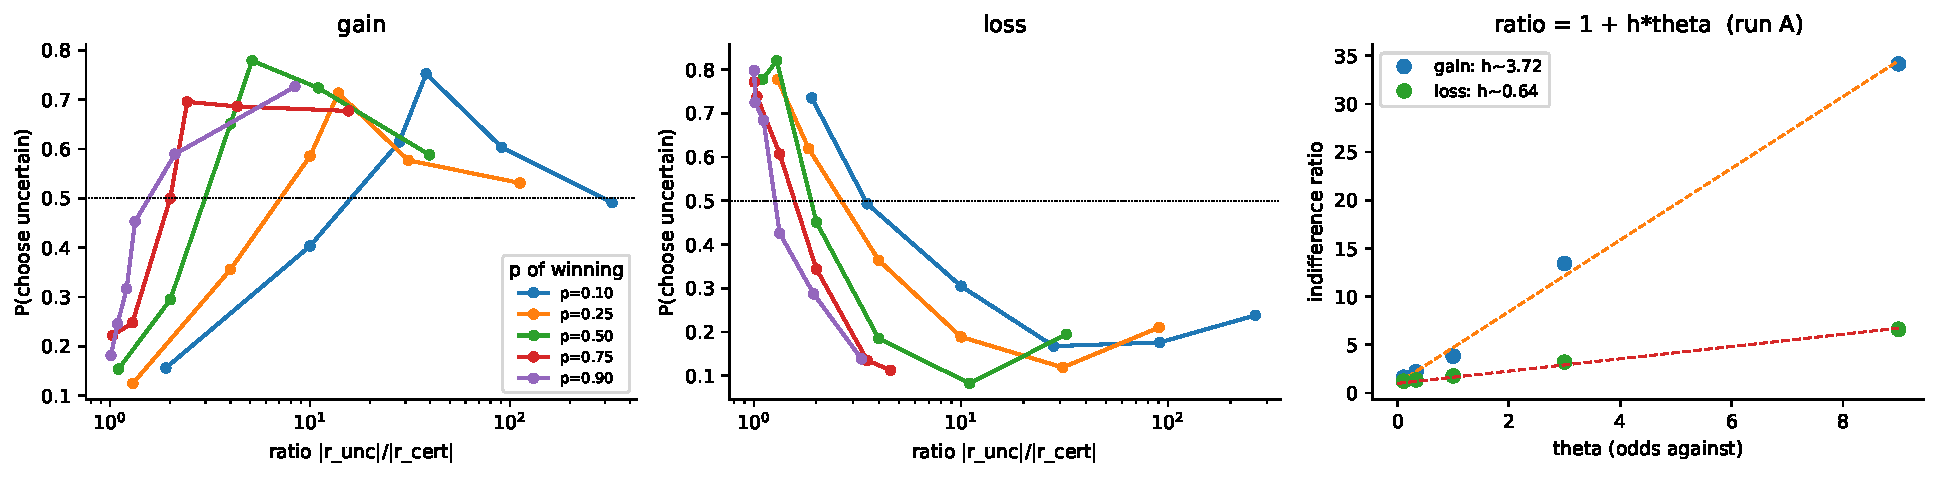
\includegraphics[width=\textwidth]{figures/fig1_data.pdf}
\caption{\textbf{Model-free data summary.} Left and middle: proportion of uncertain choices
against the magnitude ratio $|r_{unc}|/|r_{cert}|$, binned into sextiles, separately for each
outcome probability $p$, in the reward (left) and loss (middle) conditions. Right:
indifference ratios estimated at each $p$ against the odds against $\Theta$. The hyperboloid
predicts $r_{unc}/r_{cert}=1+h\Theta$ (dashed lines), giving model-free $h\approx3.24$ for
gains and $h\approx0.35$ for losses.}
\label{fig:data}
\end{figure}

\begin{figure}[H]\centering
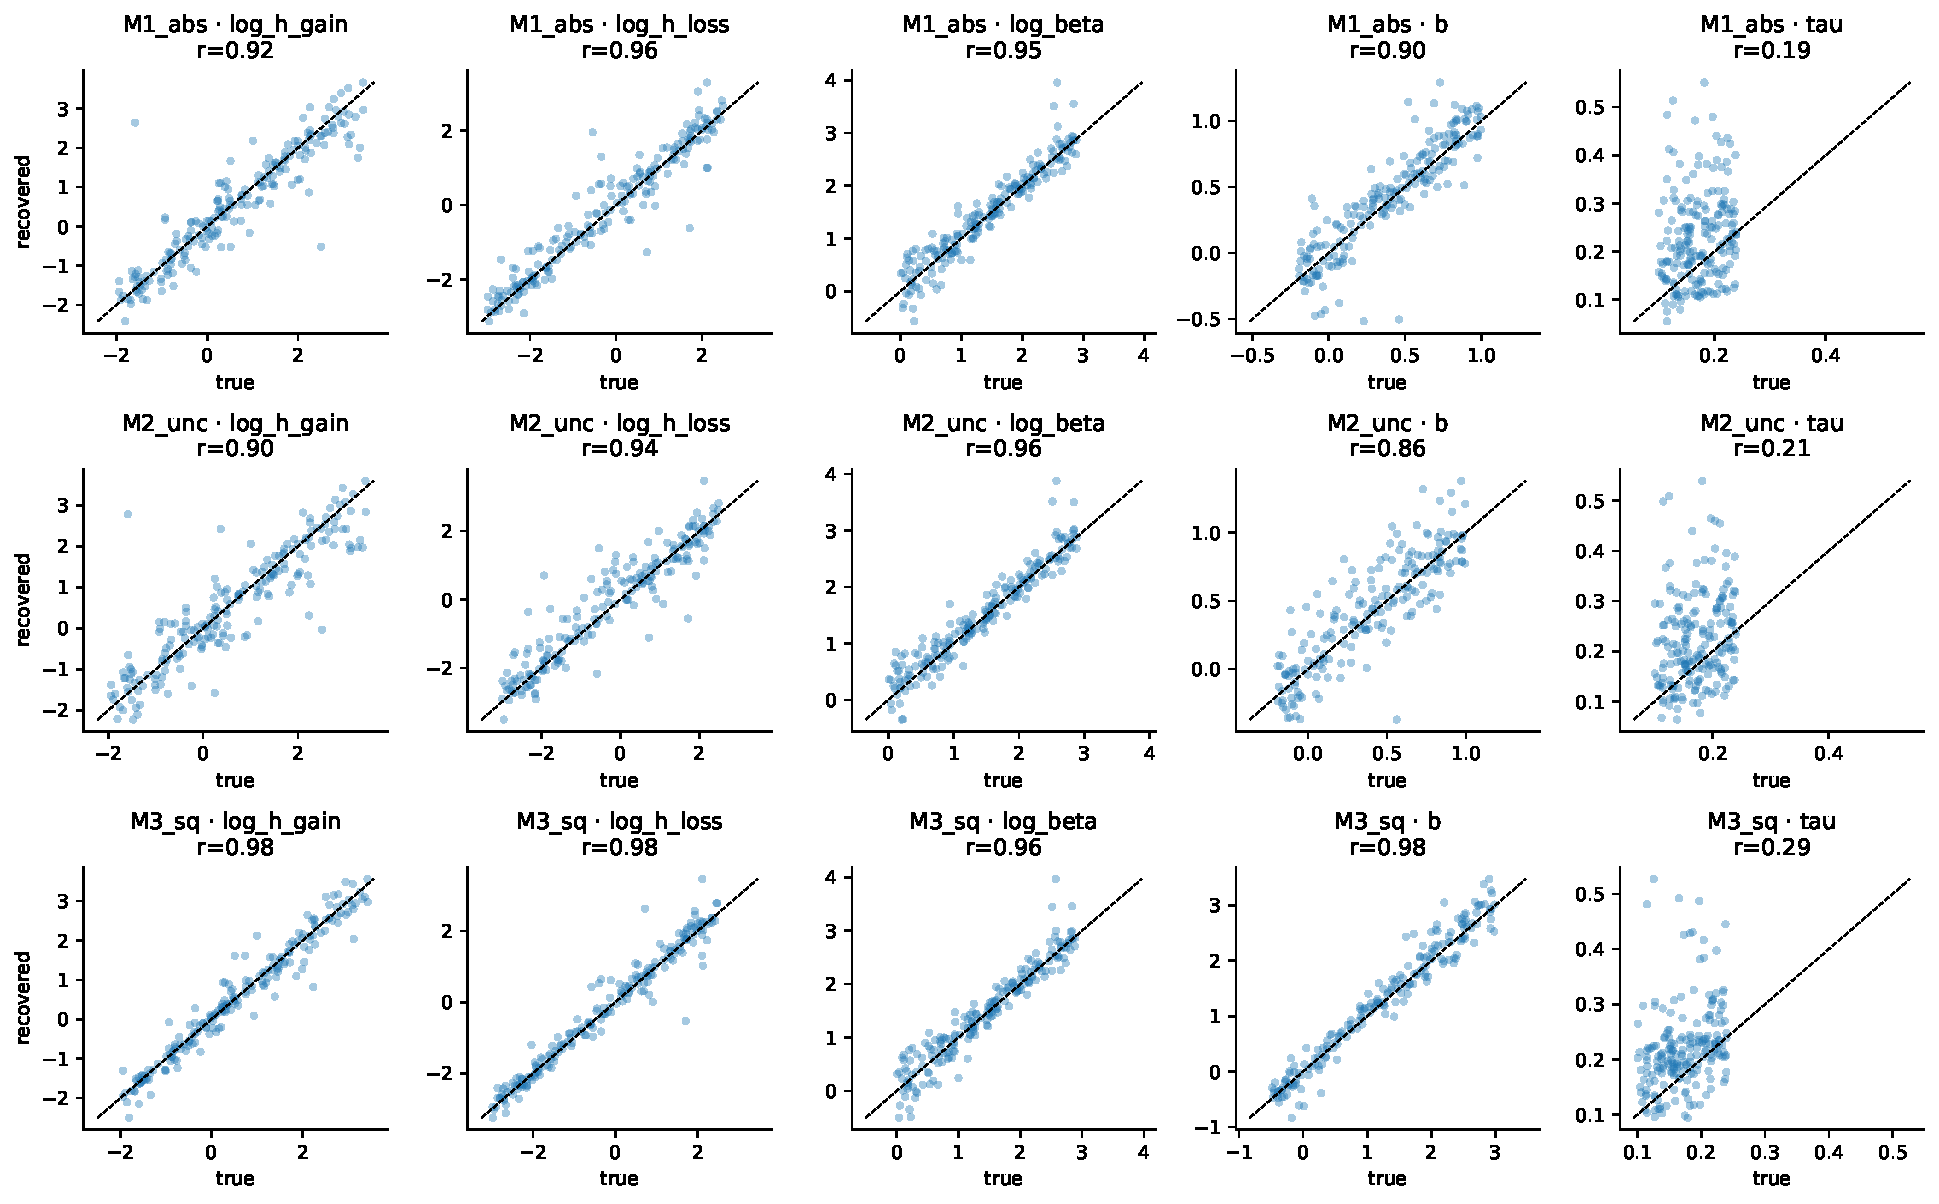
\includegraphics[width=\textwidth]{figures/fig3_recovery.pdf}
\caption{\textbf{Parameter recovery.} True against recovered values over 200 simulated
participants per model (rows: M1, M2, M3) for the two discount rates, choice sensitivity, the
difficulty slope $b$ and non-decision time $\tau$. Dashed line is identity. All choice
parameters recover well; $\tau$ does not ($r=0.19$--$0.29$).}
\label{fig:recovery}
\end{figure}

\begin{figure}[H]\centering
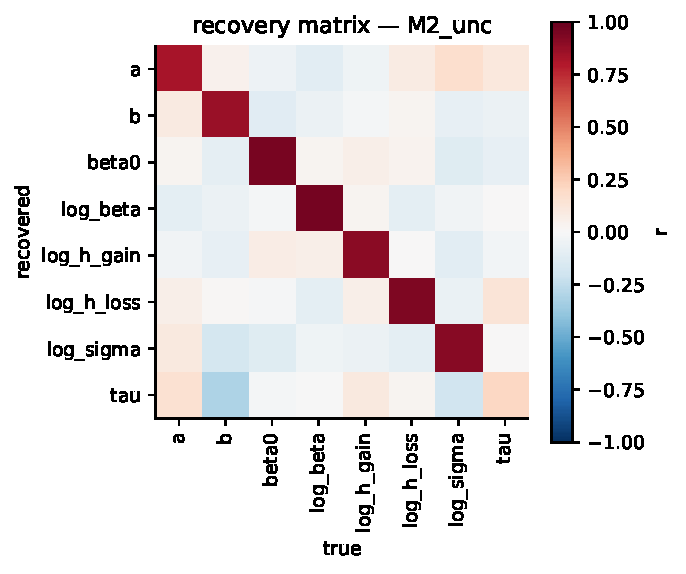
\includegraphics[width=0.55\textwidth]{figures/fig4_recovery_matrix.pdf}
\caption{\textbf{Recovery matrix (M2).} Correlation between each true parameter (columns) and
each recovered parameter (rows). Off-diagonal structure indicates trade-offs; the only
appreciable one is $\tau$ against $b$ and $a$.}
\label{fig:recmatrix}
\end{figure}

\begin{figure}[H]\centering
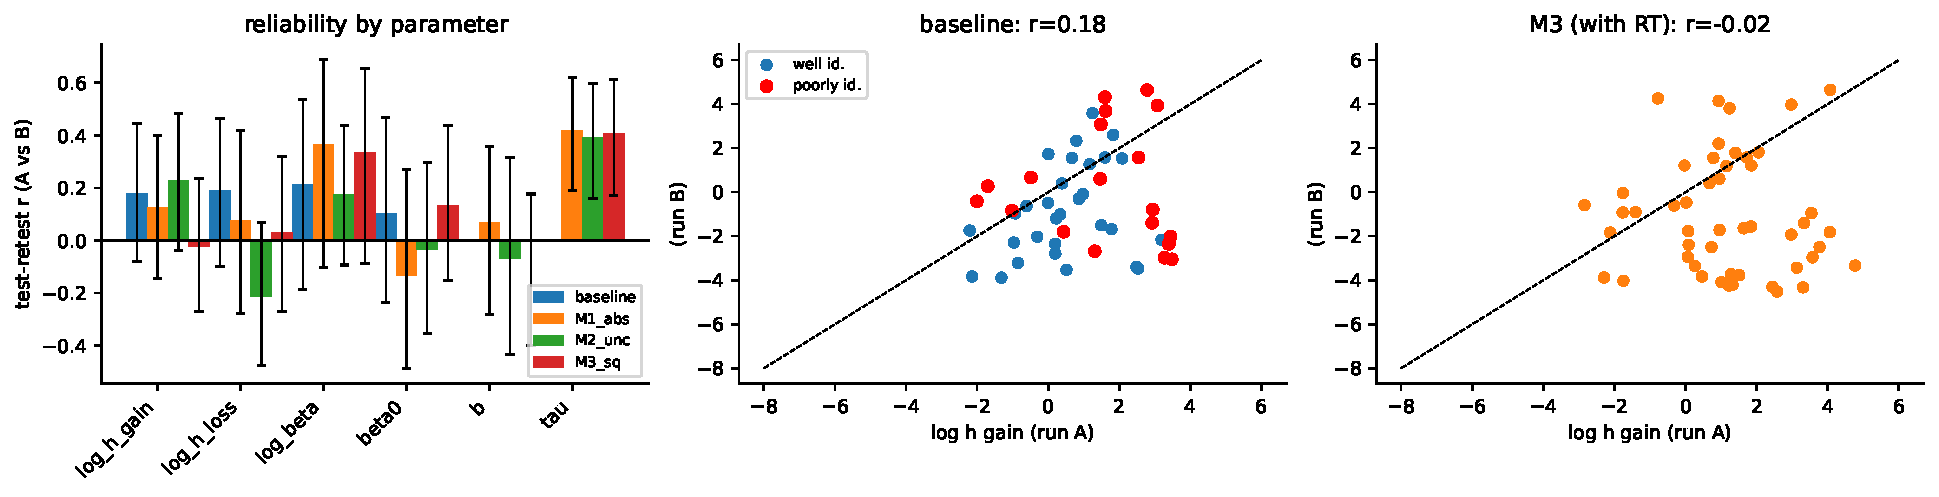
\includegraphics[width=\textwidth]{figures/fig5_reliability.pdf}
\caption{\textbf{Test--retest reliability (run A against run B).} Left: reliability per
parameter and model with bootstrap 95\% CIs. Middle and right: run A against run B estimates
of $\log h_{gain}$ for the choice-only baseline (red marks participants flagged as poorly
identified by the curvature diagnostic) and for M1, illustrating the loss of stability when RT
is added under the linear mapping.}
\label{fig:reliability}
\end{figure}

\begin{figure}[H]\centering
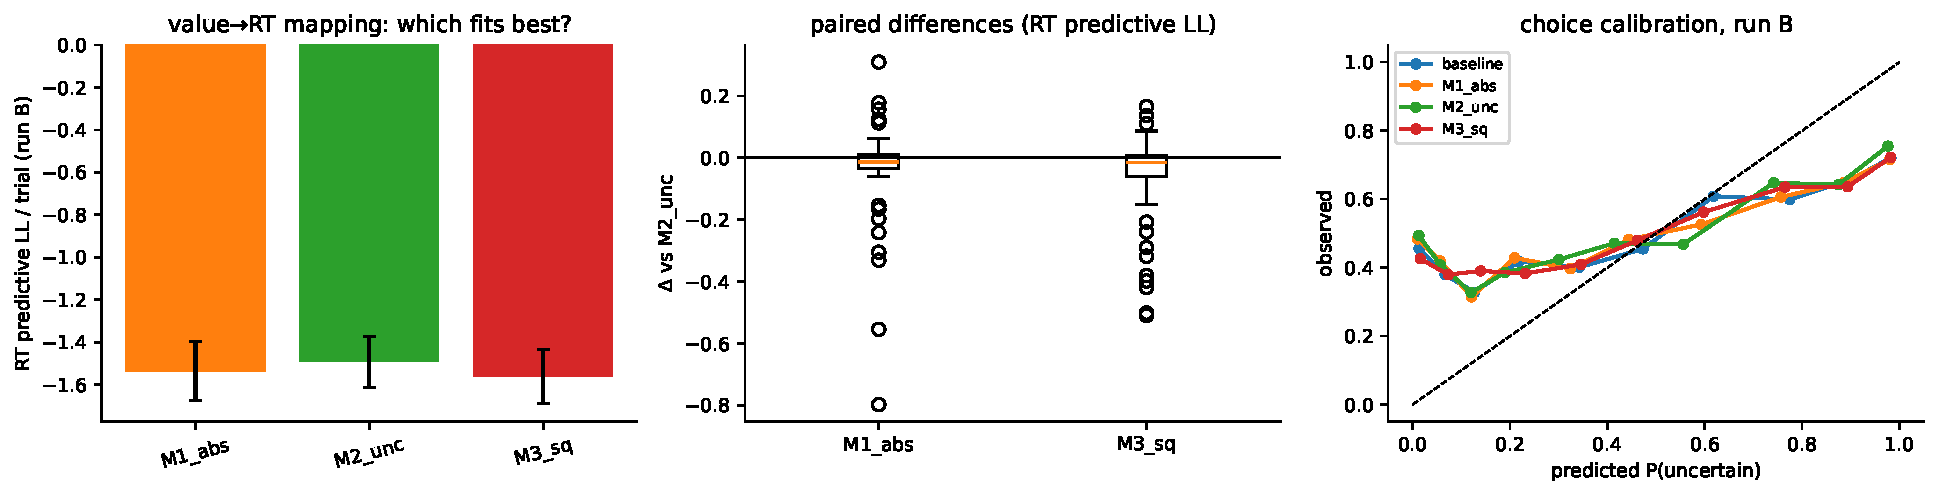
\includegraphics[width=\textwidth]{figures/fig6_prediction.pdf}
\caption{\textbf{Out-of-sample prediction (run B).} Left: RT predictive log-likelihood per
trial by model (mean $\pm$ SEM across participants), the common quantity on which the RT
models are compared. Middle: paired per-participant differences against the nominally best
model. Right: calibration of predicted against observed choice probability, decile-binned.}
\label{fig:prediction}
\end{figure}

\begin{figure}[H]\centering
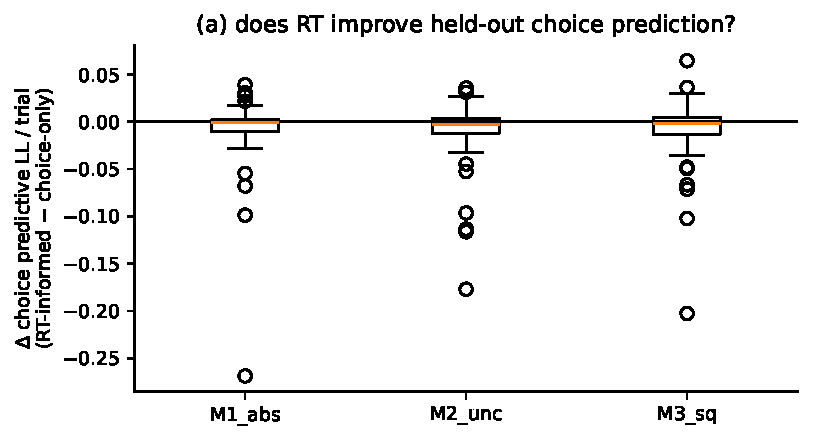
\includegraphics[width=0.5\textwidth]{figures/fig7_rt_choice.pdf}\\[6pt]
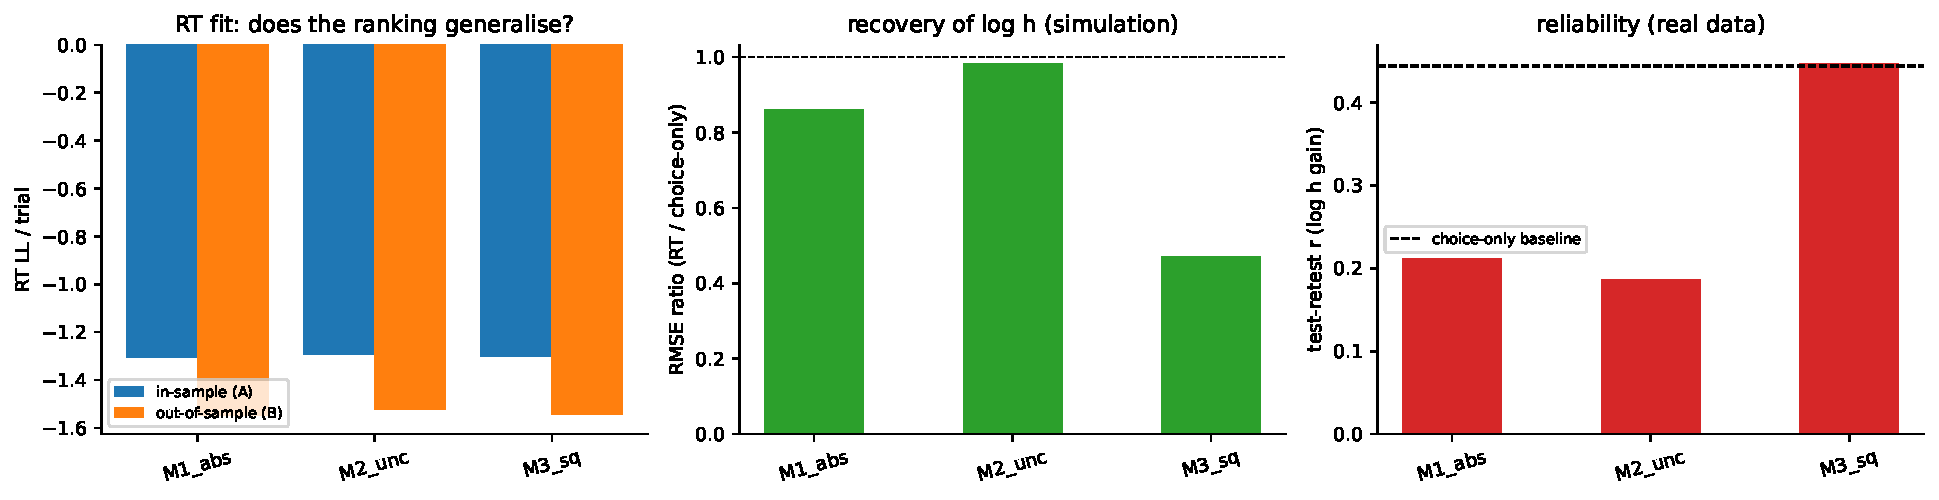
\includegraphics[width=\textwidth]{figures/fig8_evidence.pdf}
\caption{\textbf{Value of the RT modality.} Top: per-participant difference in run B choice
predictive log-likelihood between each RT-informed fit and the choice-only baseline; values
below zero mean RT hurts choice prediction. Bottom left: in-sample against out-of-sample RT
fit, showing both that the run A ranking does not generalise and how much every model loses
between sessions. Bottom middle: recovery RMSE ratio against the choice-only fit, where below
the dashed line means RT improves recovery. Bottom right: test--retest reliability of
$\log h_{gain}$ per RT model against the choice-only baseline (dashed).}
\label{fig:value}
\end{figure}

\clearpage
\section*{Tables}

\begin{table}[H]\centering
\caption{Priors on the fitted (transformed) scale, and their rationale.}
\label{tab:priors}
\small
\begin{tabularx}{\textwidth}{llX}
\toprule
Parameter & Prior & Rationale\\
\midrule
\texttt{log\_h\_gain}, \texttt{log\_h\_loss} & $\cN(0,2^2)$ & Centred at $h=1$, with 95\% mass over $h\in[0.02,55]$, far wider than the model-free estimates ($3.24$, $0.35$), so the data dominate.\\
\texttt{log\_beta} & $\cN(1,1.5^2)$ & Covers $\beta\in[0.14,52]$; excludes only numerically degenerate values.\\
\texttt{beta0} & $\cN(0,2^2)$ & No stance on the direction of bias.\\
\texttt{a} & $\cN(0.5,1^2)$ & Centred near $\log(\text{median RT}-\tau)\approx0.6$.\\
\texttt{b} & $\cN(0,1^2)$; $\cN(0,3^2)$ for M3 & Centred at zero and symmetric, so a positive difficulty effect is not assumed. Widened for M3 because $\Delta V^2$ is on a smaller scale, which keeps regularisation comparable in effect rather than in raw coefficient.\\
\texttt{log\_sigma} & $\cN(-0.5,0.5^2)$ & Matches the observed spread of $\log$ RT.\\
\texttt{tau\_raw} & $\cN(0,1.5^2)$ & Nearly flat over the admissible interval $(0,\min RT)$.\\
\bottomrule
\end{tabularx}
\end{table}

\begin{table}[H]\centering
\caption{Parameter recovery over 200 simulated participants per model. $r$ and RMSE are between
true and recovered values from the full choice\,+\,RT fit; the RMSE ratio is (joint
fit)/(choice-only fit), so values below 1 mean RT improves recovery. $b$'s RMSE is not
comparable across models because the predictors are on different scales.}
\label{tab:recovery}
\small
\begin{tabular}{lccccccccc}
\toprule
& \multicolumn{3}{c}{M1 (linear)} & \multicolumn{3}{c}{M2 (uncertainty)} & \multicolumn{3}{c}{M3 (quadratic)}\\
\cmidrule(lr){2-4}\cmidrule(lr){5-7}\cmidrule(lr){8-10}
Parameter & $r$ & RMSE & ratio & $r$ & RMSE & ratio & $r$ & RMSE & ratio\\
\midrule
$\log h_{gain}$ & 0.925 & 0.569 & 0.862 & 0.900 & 0.649 & 0.983 & \textbf{0.977} & 0.319 & \textbf{0.471}\\
$\log h_{loss}$ & 0.958 & 0.486 & 0.719 & 0.936 & 0.598 & 0.883 & \textbf{0.978} & 0.357 & \textbf{0.490}\\
$\log\beta$     & 0.955 & 0.266 & 0.964 & 0.958 & 0.253 & 0.917 & 0.956 & 0.263 & 0.923\\
$\beta_0$       & 0.954 & 0.371 & 0.869 & 0.952 & 0.382 & 0.895 & 0.963 & 0.326 & 0.760\\
$a$             & 0.884 & 0.107 & --    & 0.825 & 0.145 & --    & 0.928 & 0.086 & --\\
$b$             & 0.897 & 0.184 & --    & 0.860 & 0.210 & --    & 0.978 & 0.238 & --\\
$\log\sigma$    & 0.917 & 0.097 & --    & 0.914 & 0.098 & --    & 0.935 & 0.088 & --\\
$\tau$          & \textcolor{red}{0.187} & 0.110 & -- & \textcolor{red}{0.207} & 0.103 & -- & \textcolor{red}{0.287} & 0.089 & --\\
\bottomrule
\end{tabular}
\end{table}

\begin{table}[H]\centering
\caption{Test--retest reliability (Pearson $r$ between run A and run B estimates, $n=49$).
$\Delta$ is the difference from the choice-only baseline, and bracketed values are bootstrap
95\% CIs on that difference (2000 resamples, paired across models). Dashes mark parameters
that do not exist in the baseline.}
\label{tab:reliability}
\small
\begin{tabular}{lccccc}
\toprule
Parameter & baseline & M1 & M2 & M3 & $\Delta$M3 vs baseline\\
\midrule
$\log h_{gain}$ & 0.444 & 0.212 & 0.187 & \textbf{0.447} & $+0.003$ $[-0.21,+0.23]$\\
$\log h_{loss}$ & 0.124 & 0.118 & 0.099 & \textbf{0.304} & $+0.180$ $[-0.04,+0.40]$\\
$\log\beta$     & 0.575 & 0.560 & 0.504 & 0.532 & $-0.043$\\
$\beta_0$       & 0.361 & 0.092 & 0.164 & 0.276 & $-0.085$\\
$a$             & --    & 0.682 & 0.617 & 0.727 & --\\
$b$             & --    & 0.089 & 0.200 & 0.100 & --\\
$\log\sigma$    & --    & 0.666 & 0.671 & 0.669 & --\\
$\tau$          & --    & 0.414 & 0.391 & 0.407 & --\\
\bottomrule
\end{tabular}
\end{table}

\begin{table}[H]\centering
\caption{Out-of-sample performance on run B, participant means. Run A parameters are applied
unchanged. RT models are compared with each other on $\mathrm{LL}_{RT}$ only; RT-informed fits
are compared with the baseline on $\mathrm{LL}_{choice}$ and balanced accuracy only. All
log-likelihoods are per trial, and chance for choice is $-0.693$.}
\label{tab:prediction}
\small
\begin{tabular}{llccccc}
\toprule
Model & Condition & $\mathrm{LL}_{choice}$ & bal.\ acc. & AUC & $\mathrm{LL}_{RT}$ & RMSE $\log$RT\\
\midrule
baseline & all    & $\mathbf{-0.630}$ & \textbf{0.699} & \textbf{0.756} & -- & --\\
         & reward & $-0.637$ & 0.689 & 0.744 & -- & --\\
         & loss   & $-0.623$ & 0.697 & 0.767 & -- & --\\
\midrule
M1 & all    & $-0.640$ & 0.692 & 0.752 & $-1.548$ & 0.775\\
   & reward & $-0.650$ & 0.690 & 0.746 & $-1.616$ & 0.794\\
   & loss   & $-0.629$ & 0.690 & 0.770 & $\mathbf{-1.481}$ & 0.741\\
\midrule
M2 & all    & $-0.643$ & 0.690 & 0.750 & $\mathbf{-1.524}$ & 0.761\\
   & reward & $-0.651$ & 0.683 & 0.739 & $\mathbf{-1.546}$ & 0.769\\
   & loss   & $-0.634$ & 0.692 & 0.774 & $-1.502$ & 0.740\\
\midrule
M3 & all    & $-0.640$ & 0.689 & 0.754 & $-1.544$ & 0.781\\
   & reward & $-0.646$ & 0.689 & 0.749 & $-1.596$ & 0.797\\
   & loss   & $-0.633$ & 0.687 & 0.764 & $-1.492$ & 0.748\\
\bottomrule
\end{tabular}
\end{table}

\clearpage
\begin{thebibliography}{99}

\bibitem[Dai \& Busemeyer(2014)]{dai2014}
Dai, J., \& Busemeyer, J.~R. (2014). Towards a probabilistic, dynamic, and attribute-wise model
of intertemporal choice. \emph{Journal of Experimental Psychology: General}, 143(4),
1489--1514.

\bibitem[Enkavi et al.(2019)]{enkavi2019}
Enkavi, A.~Z., Eisenberg, I.~W., Bissett, P.~G., Mazza, G.~L., MacKinnon, D.~P., Marsch,
L.~A., \& Poldrack, R.~A. (2019). Large-scale analysis of test--retest reliabilities of
self-regulation measures. \emph{Proceedings of the National Academy of Sciences}, 116(12),
5472--5477.

\bibitem[Green \& Myerson(2004)]{green2004}
Green, L., \& Myerson, J. (2004). A discounting framework for choice with delayed and
probabilistic rewards. \emph{Psychological Bulletin}, 130(5), 769--792.

\bibitem[Hedge et al.(2018)]{hedge2018}
Hedge, C., Powell, G., \& Sumner, P. (2018). The reliability paradox: why robust cognitive
tasks do not produce reliable individual differences. \emph{Behavior Research Methods},
50(3), 1166--1186.

\bibitem[Kahneman \& Tversky(1979)]{kahneman1979}
Kahneman, D., \& Tversky, A. (1979). Prospect theory: an analysis of decision under risk.
\emph{Econometrica}, 47(2), 263--291.

\bibitem[Krajbich et al.(2010)]{krajbich2010}
Krajbich, I., Armel, C., \& Rangel, A. (2010). Visual fixations and the computation and
comparison of value in simple choice. \emph{Nature Neuroscience}, 13(10), 1292--1298.

\bibitem[Rachlin et al.(1991)]{rachlin1991}
Rachlin, H., Raineri, A., \& Cross, D. (1991). Subjective probability and delay.
\emph{Journal of the Experimental Analysis of Behavior}, 55(2), 233--244.

\bibitem[Ratcliff(1978)]{ratcliff1978}
Ratcliff, R. (1978). A theory of memory retrieval. \emph{Psychological Review}, 85(2),
59--108.

\bibitem[Ratcliff \& McKoon(2008)]{ratcliff2008}
Ratcliff, R., \& McKoon, G. (2008). The diffusion decision model: theory and data for
two-choice decision tasks. \emph{Neural Computation}, 20(4), 873--922.

\bibitem[Rodriguez et al.(2014)]{rodriguez2014}
Rodriguez, C.~A., Turner, B.~M., \& McClure, S.~M. (2014). Intertemporal choice as discounted
value accumulation. \emph{PLoS ONE}, 9(2), e90138.

\bibitem[Shrout \& Fleiss(1979)]{shrout1979}
Shrout, P.~E., \& Fleiss, J.~L. (1979). Intraclass correlations: uses in assessing rater
reliability. \emph{Psychological Bulletin}, 86(2), 420--428.

\end{thebibliography}

\end{document}
